\subsection{\href{http://www.wolfcut.es/}{Wolfcut}}
   \hypertarget{subsec:wolfcut}
I've developed a HTML/WIFI remote control for a NK105 based CNC machine for Wolfcut.\\
I've used a Beagle Bone Green Wireless embedded computer that behaves as an USB mass storage for file exchange eliminating the need of connecting and disconnecting a pendrive.\\
I've design a small Beagle break board that connect in between the keyboard cable and emulate the actual keyboard.\\
I've compiled the GCC for the ARM using crosstool-ng, then compile the linux kernel using the GCC generated, a custom file system using buildroot.\\
I've used the new style configFS to emulate the mass storage profile, and configured an apache deamon for the web GUI and php support for the backend interacion with a C code that do the actual communication with the NK105.\\
   Figura \ref{fig:wolfcut_capas} shows the implemented layer model and some captures of the web page.\\
     \begin{figure}
      \begin{center}
         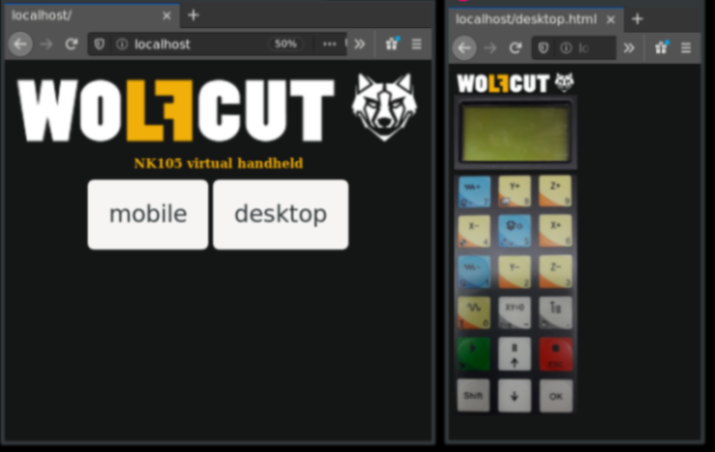
\includegraphics[width=0.3\textwidth]{wolfcut1.png}
         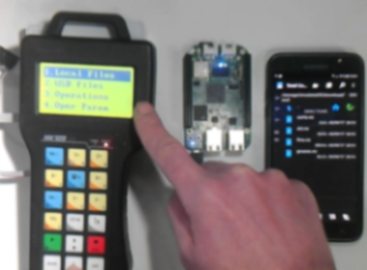
\includegraphics[width=0.3\textwidth]{wolfcut2.png}
         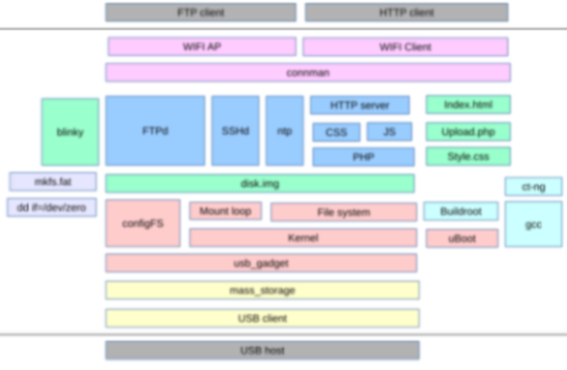
\includegraphics[width=0.3\textwidth]{wolfcut3.png}
      \end{center}
      \caption{Software layer model and the web page designed to remote control the NK105 CNC controller through WIFI.}
      \label{fig:wolfcut_capas}
   \end{figure}

   Figure \ref{fig:wolfcut_implementacion} shows some captures of the compilation setup in action.\\

     \begin{figure}
      \begin{center}
         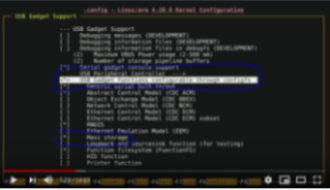
\includegraphics[width=0.3\textwidth]{wolfcut4.png}
         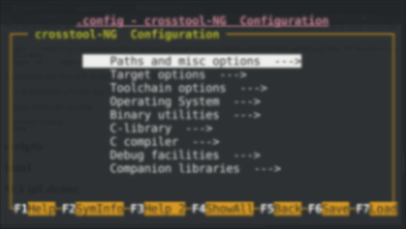
\includegraphics[width=0.3\textwidth]{wolfcut5.png}
         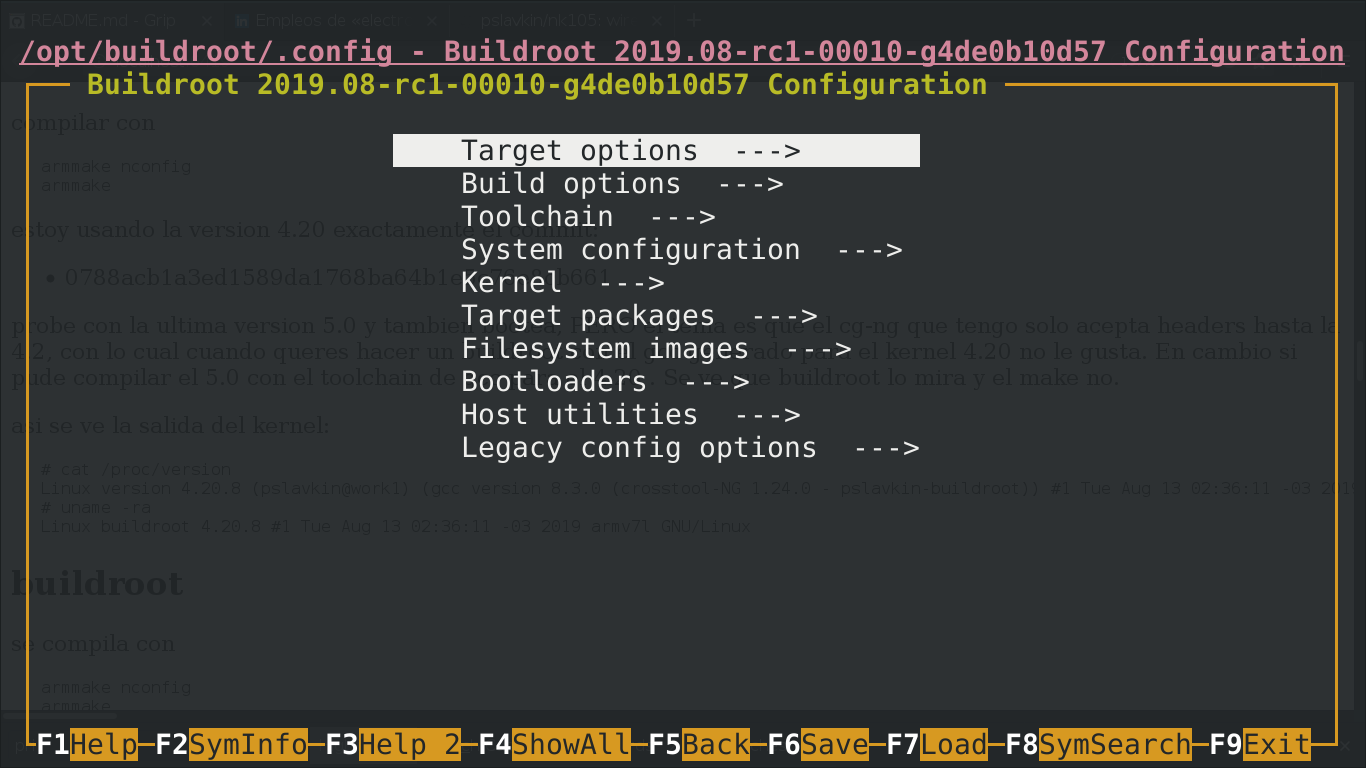
\includegraphics[width=0.3\textwidth]{wolfcut6.png}
      \end{center}
      \caption{crosstool-ng, kernel and buildroot setup, used in the wifi remote control of NK105}
      \label{fig:wolfcut_implementacion}
   \end{figure}
